\documentclass{beamer}
\usepackage{amsfonts, amsmath, graphicx, verbatim, graphicx, hyperref,
  color}
\definecolor{UNBlue}{RGB}{91, 146, 229}
\setbeamercolor{structure}{fg=UNBlue}
\newcommand\Fontvi{\fontsize{6.5}{7.2}\selectfont}
\usetheme{Warsaw}

\title{Flag Aggregation and Much More ...}
\author{\it Michael C. J. Kao}
\institute{Food and Agriculture Organization \\ of the United Nations}
\date{}

\AtBeginSection[]
{
  \begin{frame}<beamer>
    \frametitle{Outline for section \thesection}
    \tableofcontents[currentsection]
  \end{frame}
}

\begin{document}

\frame{
  \titlepage
  \centering
  
\includegraphics[scale = 0.2]{fao_logo.png}
}

\frame{
  \frametitle{Outline}
  \tableofcontents
}


\section{Introduction}

\frame{
  \frametitle{Background}

  Since the introduction of the new Statistical Working System (SWS),
  many innovative approaches has been devised to improve the current
  status and to accomodate for future needs of the fast changing world
  of statistics.

  \vfill

  One subtle yet fundamental change is the separation of a single
  symbol into two separate flag. A symbol or flag is a meta data which
  indicate the collection or methodological procedure that generates
  the value.

  \vfill

  The aim of this presentation is to introduce the change and how the
  observation status flag can impact future works.

}

\frame{
  \frametitle{Mixing of Status and Method}

  Historically, a symbol can represent how it was calculated, or where
  it was is collected. However, this mixed approach has created some
  confusion and loss of information.

  \vfill
  
  For example, when yield are calculated based on production and area
  harvested, a flag "C" representing "calculated" is
  assigned. However, it does not show the observation status of yield.

  \vfill

  A value for yield calculated based on official data has the same
  equivalent meaning to those calculated on estimates.

  \vfill

  This mixing of information results in loss of information and
  potential bias analysis.
  
 
}


\frame{
  \frametitle{Separation of Status and Method}

  To better represent these information, the decision was made to
  split the symbol into two separate flag reflecting different piece
  of information.

  \vfill

  One for the \textbf{observation status} which represents how the
  data was observed, whether collected from official or semi-official
  data source, or it maybe estimated or imputed.

  \vfill

  The second flag would denote the \textbf{methodology} it was
  obtained. Official figure can be obtained from questionnaire, or it
  can be from database or publications. Value which are estimated can
  be manually derived based or algorithm driven.

}


\frame{
  \frametitle{Problem}

  Nevertheless, it presents a problem. How do we assign observation
  flag when a value is calculated? Take the yield for example again,
  we would assign a method flag indicating the value was calculated;
  but what is its observation status?
  
}


\section{Aggregation of Observation Flag}

\frame{
  \frametitle{What should the correct observation flag?}

  One approach is to quantify the believability of information for
  each flag and treating them as ordinal variables. Then the
  aggregation can be proceeded by taking the lower bounds of the set.

  \vfill

  The rational for that is that the believability of an aggregation
  should reflect the lowest level of believability.

  %% It's like aggregating two different distribution. We have to take
  %% the variance.

}

\frame{
  \frametitle{The Flag Table}

  Shown below are the weights used to rank the flags.

  \begin{table}[h!]
    \begin{center}
      \caption{Description of the Observation flag}
      \begin{tabular}{|c|c|p{5cm}|}
        \hline
        Flags & Weights & Description\\
        \hline
        (blank) & 1 & Official Figure\\
        T & 0.8 & Unofficial figure\\
        E & 0.75 & Estimates\\
        I & 0.5 & Imputed\\
        M & 0 & Missing\\
        \hline
      \end{tabular}
    \end{center}  
  \end{table}
  

}


\frame{
  \frametitle{An example}
  
  Given that the yield is computed based on production and area
  harvested, then the observation flag should only depend on the flag
  of production and area harvested and is the minimum of the two.

  \vfill

  Lets assume that official figure are of higher quality than
  unofficial sources. Then the flag of yield computed from a
  production collected from official survey and area harvested
  collected from unofficial database should be unofficial.

}


%% \frame{
%%   \frametitle{}
%% }



\section{Potential Applications}
\frame{
  \frametitle{}
  
  The recognition of various data source and quantification of the
  believability provides many potential application which can improve
  the quality of overall statistics.

}


\frame{
  \frametitle{Robust From Outlier}
  %% include graphics on robust fitting

  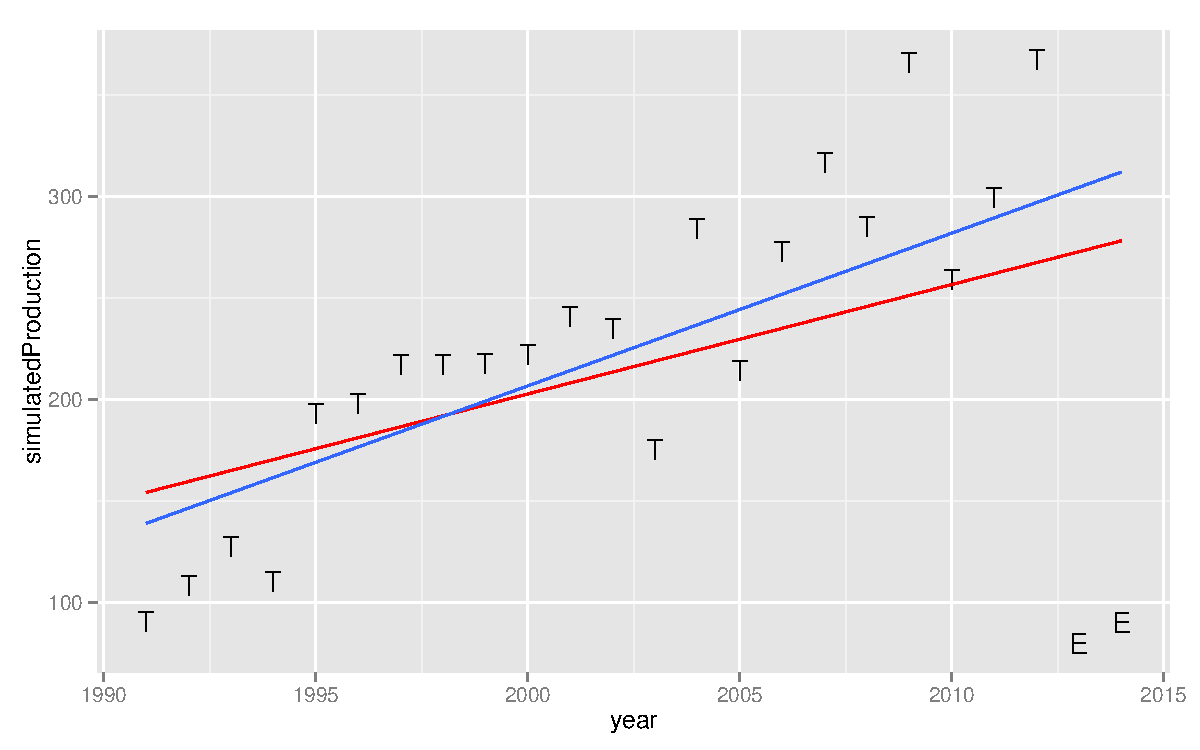
\includegraphics[scale=0.5]{robust.pdf}
}


\frame{
  \frametitle{Combining Source of Different Information Quality}
  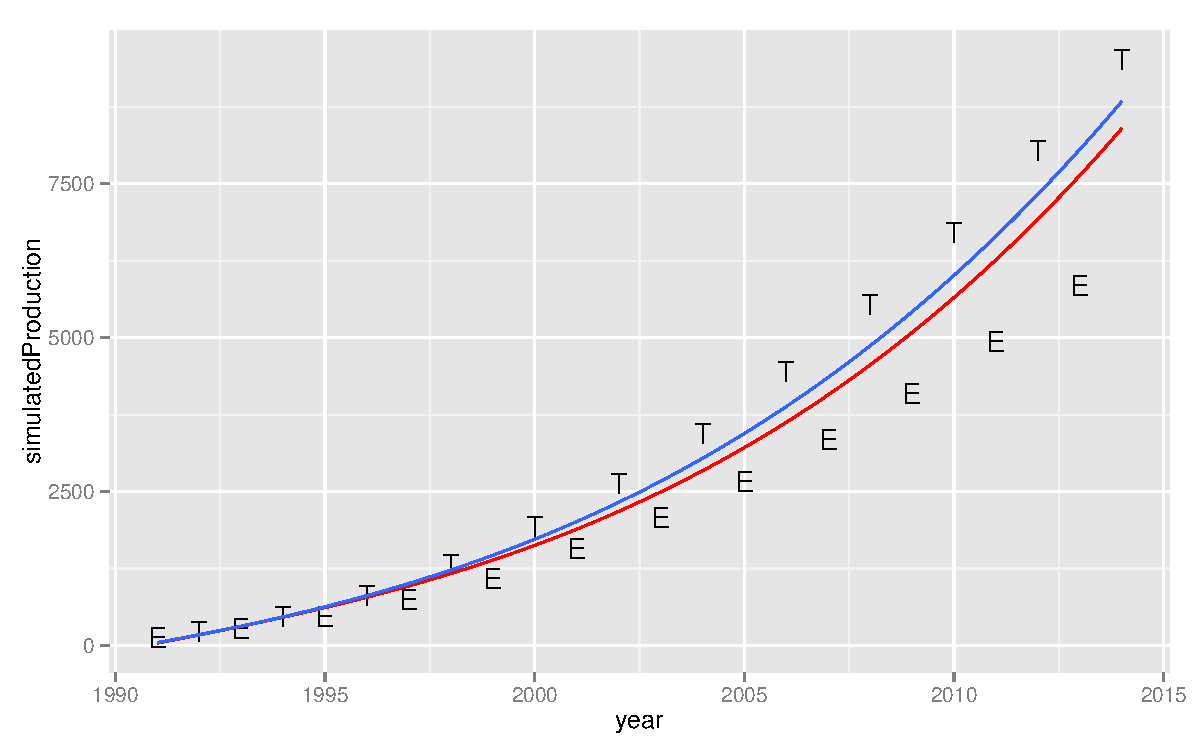
\includegraphics[scale=0.5]{combine.pdf}
  %% Include figure on combining different sources

}


\frame{
  \frametitle{}
  
  The potential associated with quantifying the quality of information
  is huge. It provides an additional piece of information for every
  single data point.

  \vfill
  
  This is a general framework, no specific methodology is required
  since any model and methodology can utilize this framework by
  incorporate the additional information.

}


\section{Computing Weights}


\frame{
  \frametitle{}

  Currently, the weights are assigned subjectively by expert
  judgements in order to preserve a rank order.

  \begin{table}[h!]
    \begin{center}
      \caption{Description of the Observation flag}
      \begin{tabular}{|c|c|p{5cm}|}
        \hline
        Flags & Weights & Description\\
        \hline
        (blank) & 1 & Official Figure\\
        T & 0.8 & Unofficial figure\\
        E & 0.75 & Estimates\\
        I & 0.5 & Imputed\\
        M & 0 & Missing\\
        \hline
      \end{tabular}
    \end{center}  
  \end{table}
  
  However, methods are being devised to estimate these weights
  objectively and automatically.

}


\frame{
  \frametitle{}
  
  A requirement for automatized and objective computation of weights
  is required due to the fact that we do not have the human resources
  to devote to assigning weights for each country, each agricultural
  domain and partition of the data.

  \vfill

  Below we present two methods that are under-investigation for
  discussion.

}
  

\frame{
  \frametitle{Measuring Loss of Information}

  In this method, we take the official figures as gold standard. Then
  we compute the Kullback-Leibner Divergence and measure the amount of
  information loss when we represnt value in alternative sources other
  than official source.
  
  \vfill

  \begin{block}{Kullback Leibler Divergence}
    $$
    D_{\mathrm{KL}}(P\|Q) = \sum_i \ln\left(\frac{P(i)}{Q(i)}\right) P(i).\!
    $$
  \end{block}

  %% \begin{block}{Mean Squared Error}
  %%   \begin{align*}
  %%   \operatorname{MSE} &=\frac{1}{n}\sum_{i=1}^n(\hat{Y_i} - Y_i)^2\\
  %%   \omega &= \frac{MSE}{||MSE||}
  %%   \end{align*}
    
  %% \end{block}

  %% Where $Y_i$ are data from official source and $\hat{Y}$ are
  %% alternative sources. 

  %% The smaller the MSE, the greater the weight.

  The weights can then be calculated based on the relative loss of
  information. The greater amount of information lost, the lower the
  weight.

}
  

%% See if we can use AIC

\frame{
  \frametitle{Self-Similarity Weights}
  
  This alternative method does not assume which source is correct,
  rather it uses similarity between the observations of different flag
  to identify a centroid. This centroid is interpreted as close to the
  true value.
  
  \vfill

  The distance from the centroid will be inversely related to the
  weight. That is, the further away you are from the centroid, the
  lower the weight will be assigned.
  
}

\frame{
  \centering
  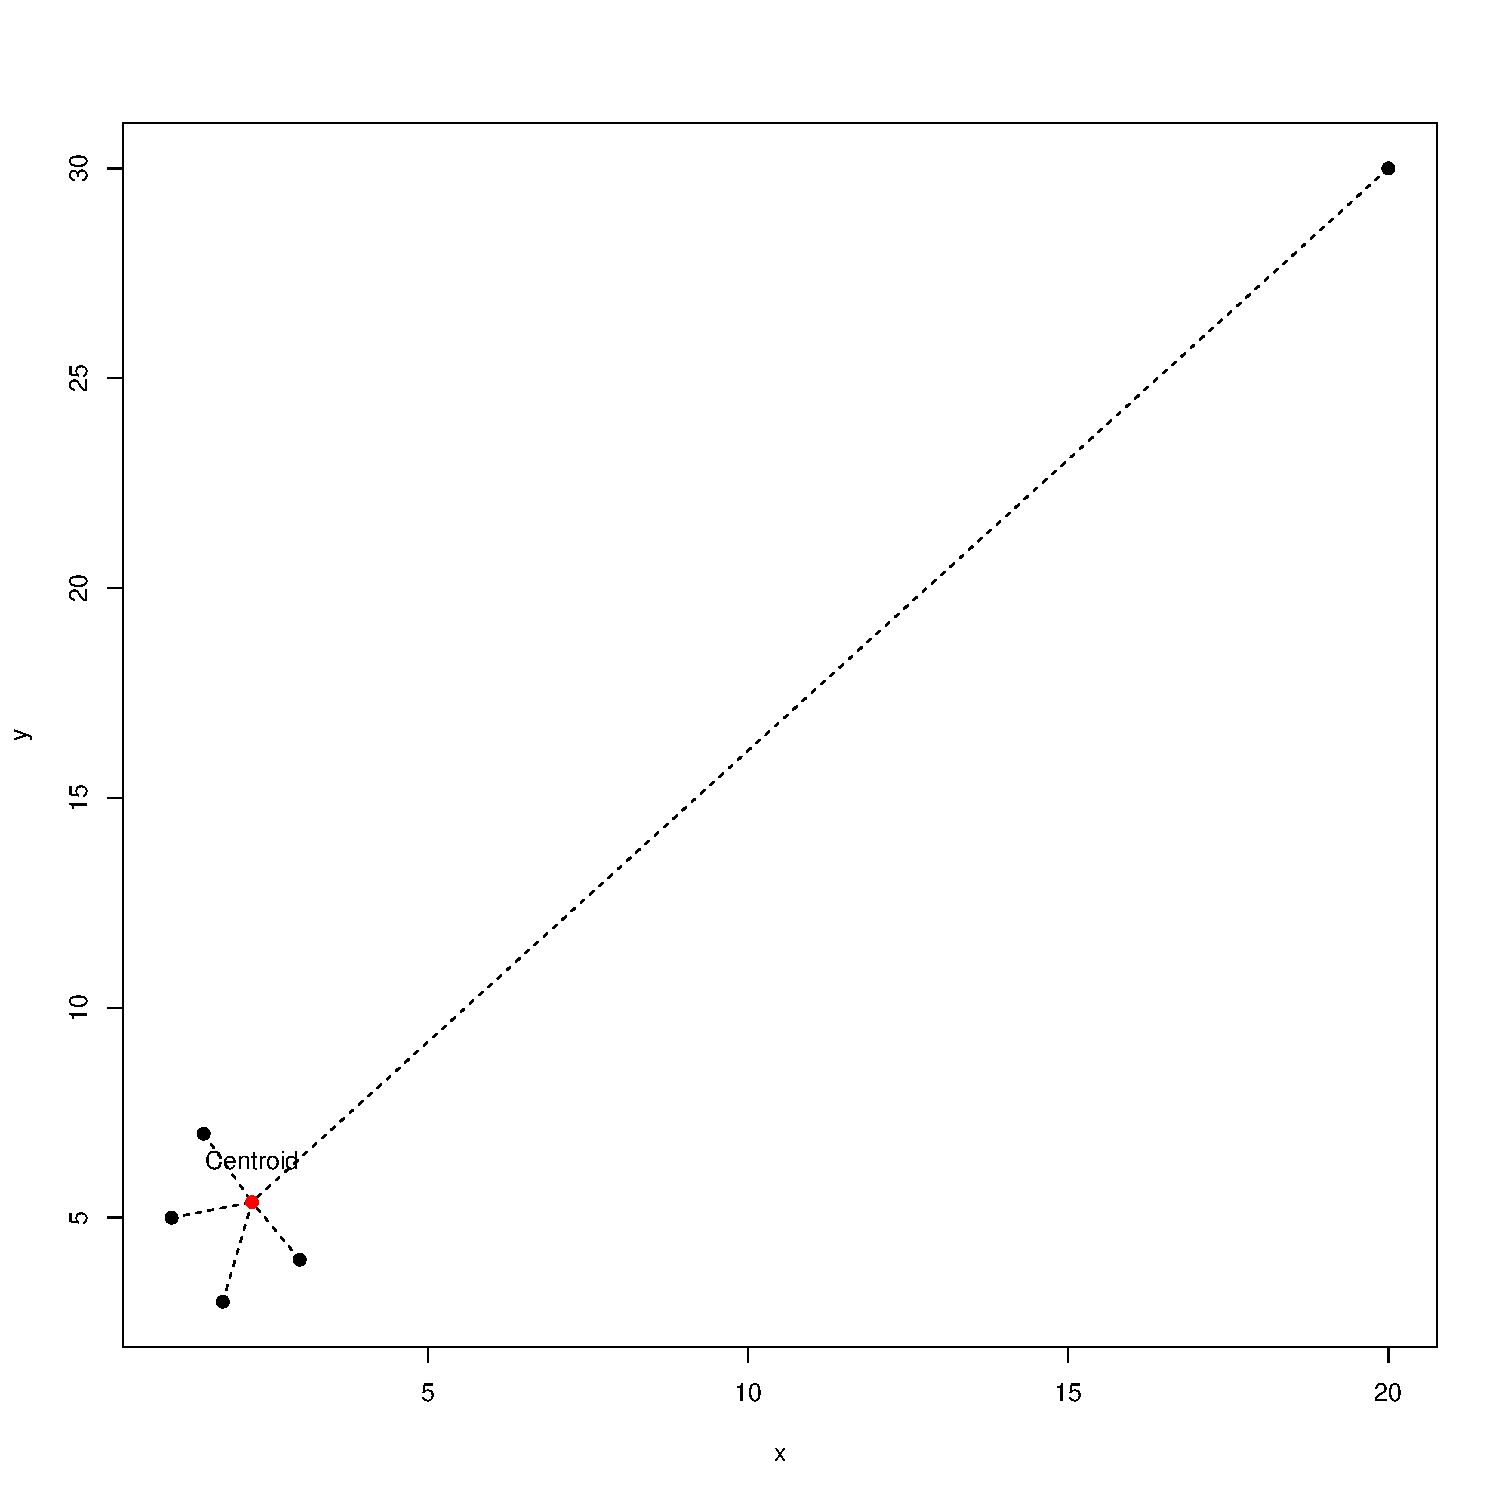
\includegraphics[scale=0.3]{centroid.pdf}
  
}  


\end{document}
